% ============================================================================
% CORRECTED + SIMPLIFIED pipeline figure (Figure 1)  -- REVIEW COPY (v2)
% Standalone & compilable (pdflatex pipeline_fixed.tex). Not committed to the
% report branch; once you approve, the tikzpicture block folds into main.tex.
%
% Design: a clean left-to-right, 4-stage flow with THREE parallel lanes (one per
% compared scorer). Straight edges only -- no sweeping arcs, no edge-label pile-ups.
%   Stage 1  shared SFT reference policy pi_ref
%   Stage 2  two conditions trained on the SAME 8k pairs (DPO, BT-RM); pi_ref kept untrained
%   Stage 3  three scorers read off
%   Stage 4  evaluation
% Correctness kept from v1: the 8k pairs train the two conditions (shown as a box line,
% not an arc), and the implicit reward reuses pi_ref (one short dashed edge, Fix 1).
% Data sizes live INSIDE the boxes, so the edges stay label-free and uncluttered.
% ============================================================================
\documentclass[11pt]{article}
\usepackage[margin=1in]{geometry}
\usepackage{amsmath}
\usepackage{tikz}
\usetikzlibrary{arrows.meta, positioning}
\usepackage{xcolor}
\usepackage{caption}
\usepackage{float}

\begin{document}

\begin{figure}[H]
\centering
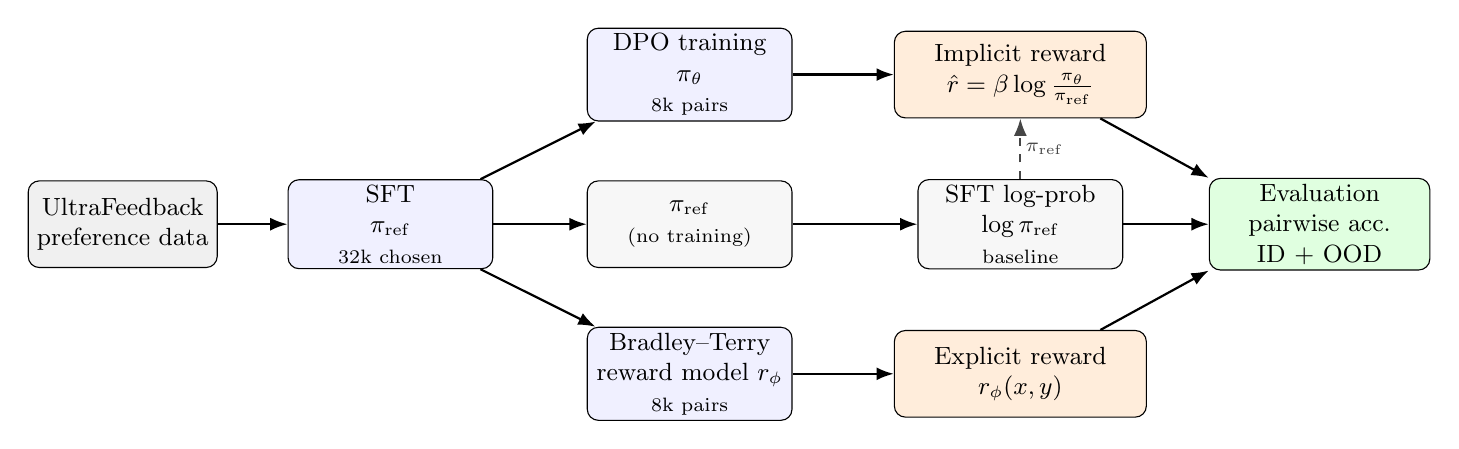
\begin{tikzpicture}[
  every node/.style={font=\small},
  box/.style={draw, rounded corners, align=center, minimum height=11mm, minimum width=26mm,
              fill=blue!6, inner sep=2pt},
  data/.style={draw, rounded corners, align=center, minimum height=11mm, minimum width=24mm,
               fill=gray!12, inner sep=2pt},
  ref/.style={draw, rounded corners, align=center, minimum height=11mm, minimum width=26mm,
              fill=gray!6, inner sep=2pt},
  reward/.style={box, fill=orange!14, minimum width=32mm},
  evalbox/.style={box, fill=green!12, minimum width=28mm},
  arr/.style={-{Latex[length=2.2mm]}, thick},
  dep/.style={-{Latex[length=2.2mm]}, thick, dashed, gray!55!black},
  deplbl/.style={font=\scriptsize\itshape, text=gray!55!black, inner sep=1.5pt}
]
  % ---- column x-positions, three lanes at y = +1.9 / 0 / -1.9 ----
  \node[data]    (data) at (0,0)      {UltraFeedback\\preference data};
  \node[box]     (sft)  at (3.4,0)    {SFT\\$\pi_{\mathrm{ref}}$\\{\scriptsize 32k chosen}};

  \node[box]     (dpo)  at (7.2,1.9)  {DPO training\\$\pi_\theta$\\{\scriptsize 8k pairs}};
  \node[ref]     (mid)  at (7.2,0)    {$\pi_{\mathrm{ref}}$\\{\scriptsize (no training)}};
  \node[box]     (rm)   at (7.2,-1.9) {Bradley--Terry\\reward model $r_\phi$\\{\scriptsize 8k pairs}};

  \node[reward]  (imp)  at (11.4,1.9) {Implicit reward\\$\hat r=\beta\log\frac{\pi_\theta}{\pi_{\mathrm{ref}}}$};
  \node[ref]     (bl)   at (11.4,0)   {SFT log-prob\\$\log\pi_{\mathrm{ref}}$\\{\scriptsize baseline}};
  \node[reward]  (exp)  at (11.4,-1.9){Explicit reward\\$r_\phi(x,y)$};

  \node[evalbox] (eval) at (15.2,0)   {Evaluation\\pairwise acc.\\ID + OOD};

  % ---- Stage 1: data -> SFT ----
  \draw[arr] (data) -- (sft);

  % ---- Stage 2: shared SFT forks into three lanes (straight) ----
  \draw[arr] (sft) -- (dpo);
  \draw[arr] (sft) -- (mid);
  \draw[arr] (sft) -- (rm);

  % ---- Stage 3: each lane yields a scorer (straight) ----
  \draw[arr] (dpo) -- (imp);
  \draw[arr] (mid) -- (bl);
  \draw[arr] (rm)  -- (exp);

  % ---- Fix 1: implicit reward reuses pi_ref (short, clean, vertical) ----
  \draw[dep] (bl) -- (imp) node[deplbl, midway, right]{$\pi_{\mathrm{ref}}$};

  % ---- Stage 4: all three scorers -> evaluation (clean fan-in) ----
  \draw[arr] (imp) -- (eval.north west);
  \draw[arr] (bl)  -- (eval.west);
  \draw[arr] (exp) -- (eval.south west);
\end{tikzpicture}
\caption{Pipeline overview (left to right). \textbf{(1)}~One SFT pass on 32k \emph{chosen}
UltraFeedback responses yields the shared reference policy $\pi_{\mathrm{ref}}$. \textbf{(2)}~From
that identical start, two conditions train on the \emph{same} 8k preference pairs, differing only
in loss --- DPO ($\to\pi_\theta$) and a Bradley--Terry reward model ($\to r_\phi$); $\pi_{
\mathrm{ref}}$ is also kept untrained. \textbf{(3)}~Three scorers are read off: the implicit
reward $\hat r=\beta\log(\pi_\theta/\pi_{\mathrm{ref}})$, which reuses $\pi_{\mathrm{ref}}$
(dashed); the explicit reward $r_\phi$; and the SFT log-probability baseline $\log\pi_{\mathrm{
ref}}$. \textbf{(4)}~All three are evaluated as pairwise preference classifiers, in distribution
and under shift.}
\label{fig:pipeline}
\end{figure}

\end{document}
